\section{Vorbereitung}
Im folgenden werden die Fourier-Koeffizienten von drei verschiedenen periodischen Schwingungsformen bestimmt. Diese dienen als Referenzwerte für die weitere Durchführung, sowie für die Auswertung des Versuches.
\subsection{Rechteckschwingung}
Für eine Rechteckschwingung lässt sich mit Hilfe der Gleichungen \eqref{eqn:an} und \eqref{eqn:bn} zeigen:
\begin{align*}
    a_n &= 0 \\
    b_n &= 
    \begin{cases}
    0 ,     & \text {für gerade $n$} \\
    \frac{C}{n} & \text {für ungerade $n$}
    \end{cases} .
\end{align*}
Da in diesem Versuch lediglich die $n$-Abhängigkeit untersucht wird, wird die Konstante $C$ nicht näher bestimmt. In Abbildung \ref{fig:vorbereitung_rechteck} ist die Funktion abgebildet, die entsteht, wenn die ersten neun Koeffizienten in das Fouriersche Theorem (Gl. \eqref{eqn:Fourier-Reihe}) eingesetzt werden.
\begin{figure}[h]
  \centering
  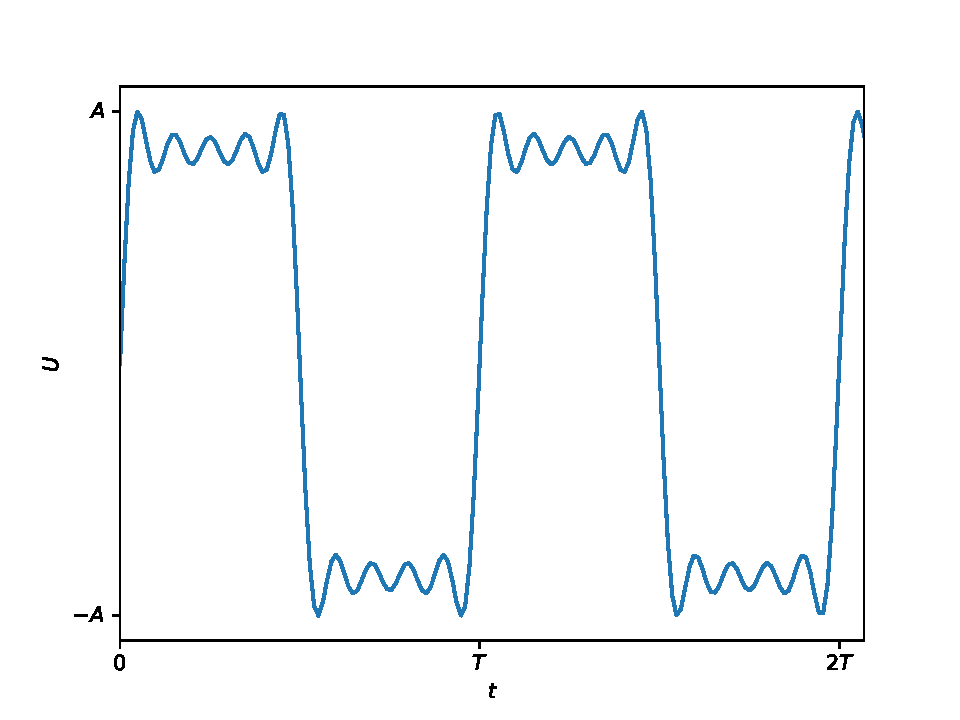
\includegraphics[width=\textwidth]{assets/fourier_rechteck.pdf}
  \caption{Fourier-Annäherung einer Rechteckschwingung für $n=9$}
  \label{fig:vorbereitung_rechteck}
\end{figure}
\subsection{Dreiecksschwingung}
Wie zuvor bei der Rechteckschwingung werden die Gleichungen \eqref{eqn:an} und \eqref{eqn:bn} benutzt, um folgende Relationen für die Fourierkoeffizienten einer Dreiecksschwingung zu zeigen:
\begin{align*}
    a_n &= 0 \\
    b_n &= 
    \begin{cases}
    0 ,     & \text {für gerade $n$} \\
    \frac{C}{n^2} & \text {für ungerade $n$}
    \end{cases} .
\end{align*}
Werden die ersten neun Koeffizienten in das Fouriersche Theorem eingesetzt, ergibt sich die Funktion, die in Abbildung \ref{fig:vorbereitung_dreieck} dargestellt ist.
\begin{figure}[h]
  \centering
  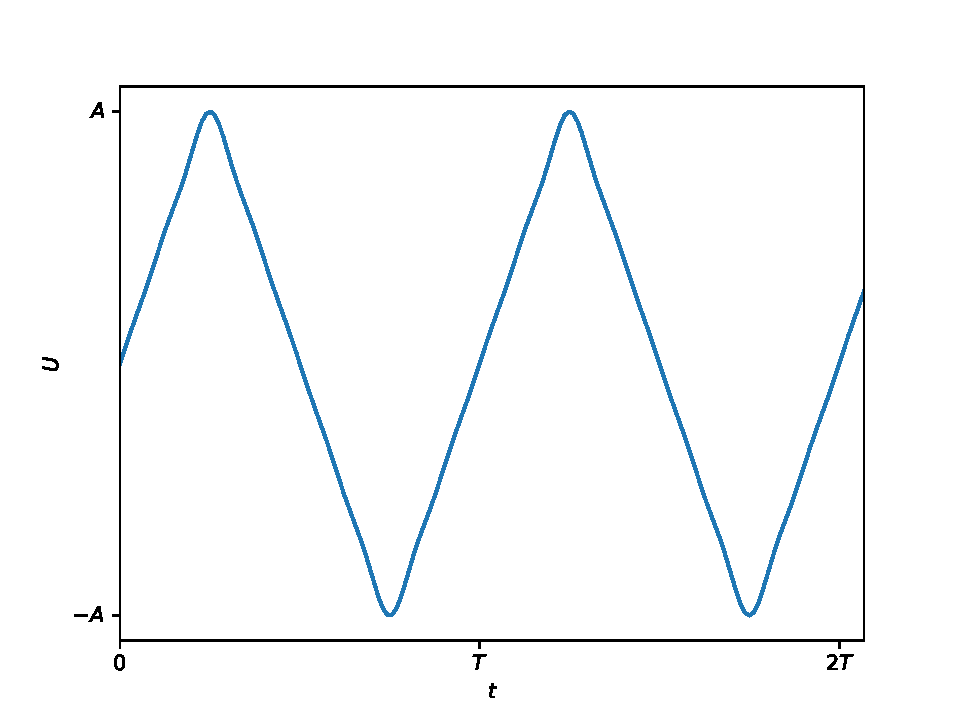
\includegraphics[width=\textwidth]{assets/fourier_dreieck.pdf}
  \caption{Fourier-Annäherung einer Dreiecksschwingung für $n=9$}
  \label{fig:vorbereitung_dreieck}
\end{figure}
\subsection{Sägezahnschwingung}
Wie zuvor sind im folgenden die mit Gleichungen \eqref{eqn:an} und \eqref{eqn:bn} bestimmten Relationen für die Sägezahnschwingung, sowie in Abbildung \ref{fig:vorbereitung_sägezahn} die Fourier-Funktion mit den ersten neun Koeffizienten aufgelistet:
\begin{align*}
    a_n &= 0 \\
    b_n &= \frac{-C}{n}
\end{align*}
\begin{figure}[h]
  \centering
  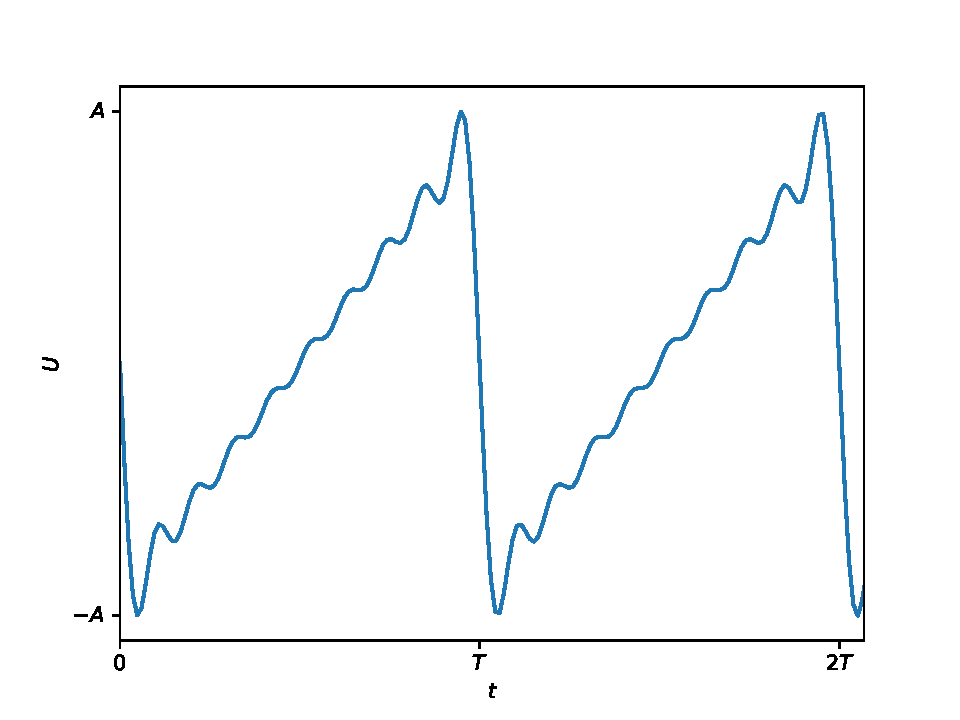
\includegraphics[width=\textwidth]{assets/fourier_zahn.pdf}
  \caption{Fourier-Annäherung einer Sägezahnschwingung für $n=9$}
  \label{fig:vorbereitung_sägezahn}
\end{figure}
